\documentclass[12pt,a4paper]{article}

% --- Packages ---
\usepackage[margin=1in]{geometry}
\usepackage{graphicx}
\usepackage{float}
\usepackage{booktabs}
\usepackage{array}
\usepackage{hyperref}
\usepackage{amsmath, amssymb}
\usepackage{enumitem}
\usepackage{lmodern}
\usepackage[T1]{fontenc}
\usepackage{textcomp}
\usepackage{titlesec}
\usepackage{subcaption}

\hypersetup{
  colorlinks=true,
  linkcolor=blue,
  urlcolor=blue
}

% --- Metadata Macros (edit these) ---
\newcommand{\university}{Politecnico di Torino}
\newcommand{\department}{Department of Control and Computer Engineering}
\newcommand{\degree}{Master's Degree in Computer Engineering}
\newcommand{\academicyear}{2025/2026}
\newcommand{\course}{Technologies for Autonomous Vehicles}
\newcommand{\reporttitle}{Assignment 1: Global Path Planning} % e.g., "Report 1"
\newcommand{\reportdate}{17/03/2026}    % or "Date, \_\_\_"

% Helper to list students as "Name Surname -- S123456"
\newcommand{\student}[2]{#1 -- #2\\}

% --- Title Page ---
\begin{document}
\begin{titlepage}
  \centering
  \vspace*{1cm}
  
\includegraphics[width=0.35\textwidth]{img/logo_poli.png}\par
  \vspace{1cm}
  {\LARGE \textbf{\university}\par}
  \vspace{0.3cm}
  {\large \department\par}
  \vspace{0.3cm}
  {\Large \degree\par}
  \vspace{0.6cm}
  {\Large \academicyear\par}
  \vspace{0.8cm}
  {\LARGE \textbf{\course}\par}
  \vspace{0.8cm}
  {\LARGE \textbf{\reporttitle}\par}
  \vfill
  {\large \reportdate \par}
  \vspace{0.2cm}
  {\large
  % --- EDIT THE NAMES BELOW ---
  \student{Fabio Veroli}{S336301}
  }
  \vspace*{0.5cm}
\end{titlepage}

\tableofcontents
\newpage

% --- Body ---

\section{Objective}

This report presents the implementation and comparative analysis of two global path planning algorithms, Dijkstra's algorithm and A*, applied to real-world road networks extracted from OpenStreetMap via the \texttt{osmnx} library.
The primary objective is to evaluate and compare the computational performance of the two algorithms in terms of the number of iterations required to find an optimal path, across two cities of significantly different scale: Aosta and Turin.

Dijkstra's algorithm is used as the baseline, as it guarantees an optimal solution on graphs with non-negative edge weights.
A* is then implemented in three variants, each employing a different heuristic function to guide the search:
\begin{itemize}
  \item \textbf{Manhattan distance} 
  \item \textbf{Euclidean distance} 
  \item \textbf{Haversine distance} 
\end{itemize}

For each algorithm and city, ten origin-destination pairs are evaluated and the average number of iterations is recorded.
The results are then discussed in relation to graph size (number of nodes and edges) and heuristic choice, with the aim of assessing the practical benefit of informed search over uninformed search.

\section{Design}

\subsection{Graph Construction}

Road networks are obtained from OpenStreetMap using the \texttt{osmnx} library.
For each city, a directed multigraph is constructed by querying the city's administrative boundary with \texttt{network\_type="drive"}, so that only road segments accessible to motor vehicles are included.
Each node represents a road junction and stores geographic coordinates (longitude and latitude), while each directed edge represents a road segment with attributes such as \texttt{length} (in metres) and \texttt{maxspeed} (in km/h).

\subsection{Edge Weight Computation}

The weight assigned to each edge models travel time rather than physical distance, as travel time is a more practical optimisation criterion for vehicle routing.
The weight is defined to represent the physical travel time in seconds:
\[
  w(e) = \frac{\ell(e)}{v_{\max}(e) / 3.6}
\]
where $\ell(e)$ is the length of edge $e$ in metres and $v_{\max}(e)$ is the posted speed limit in km/h.
Dividing the speed limit by 3.6 converts it to metres per second, ensuring dimensional consistency.
For edges where no speed limit is recorded in OpenStreetMap, a default value of 40~km/h is assumed.

\subsection{Dijkstra's Algorithm}

Dijkstra's algorithm is implemented using a binary min-heap (\texttt{heapq}) as the priority queue.
Each node maintains a \texttt{distance} label, initialised to $+\infty$ except for the source, which is set to 0.
At each iteration, the node with the smallest tentative distance is extracted; if it has already been marked as visited, it is skipped; otherwise, all outgoing neighbours are relaxed.
The algorithm terminates as soon as the destination node is extracted from the queue, guaranteeing optimality on graphs with non-negative edge weights.
The number of iterations is defined as the count of nodes successfully processed (i.e.,\ extracted and not yet visited) before termination. 

\subsection{A* Algorithm}
\label{sec:astar_design}

A* extends Dijkstra by incorporating a heuristic function $h(n)$ that estimates the remaining cost from node $n$ to the destination.
The priority of each node in the queue is:
\[
  f(n) = g(n) + h(n)
\]
where $g(n)$ is the exact travel-time cost accumulated from the source to $n$.
To ensure dimensional consistency between $g(n)$ and $h(n)$, each distance-based heuristic estimate (in metres) is normalised by the maximum speed limit $v_{\max}^{\star}$ observed in the graph:
\[
  h(n) = \frac{d(n,\, \text{dest})}{v_{\max}^{\star}}
\]
For the Euclidean and Haversine variants, this normalisation guarantees admissibility: since any road path between two nodes is at least as long as the straight-line distance between them, dividing the straight-line estimate by $v_{\max}^{\star}$ yields a strict lower bound on the remaining travel time.
The Manhattan variant uses a distance measure that satisfies $d_{\text{Man}} \geq d_{\text{Euc}}$ and therefore does not carry a formal admissibility guarantee; A* optimality is not theoretically assured when using this heuristic, and this is confirmed empirically by run~3 in Aosta (Section~\ref{sec:results_aosta}).
Three functions are used to compute the geometric distance $d$:

\begin{itemize}
  \item \textbf{Manhattan}: $d = |x_1 - x_2| + |y_1 - y_2|$, where $(x_i, y_i)$ are projected metric coordinates in metres.

  \item \textbf{Euclidean}:
  \[
    d = \sqrt{(x_1 - x_2)^2 + (y_1 - y_2)^2}
  \]
  where $(x_i, y_i)$ are projected metric coordinates in metres.
  The computation is delegated to \texttt{ox.distance.euclidean}.

  \item \textbf{Haversine}: the great-circle distance between two points on the Earth's surface,
  given their latitude $\phi$ and longitude $\lambda$ (the formula is expressed in radians; the implementation via \texttt{ox.distance.great\_circle} accepts decimal degrees and performs the conversion internally):
  \begin{align*}
    a &= \sin^2\!\left(\frac{\Delta\phi}{2}\right)
       + \cos\phi_1\,\cos\phi_2\,\sin^2\!\left(\frac{\Delta\lambda}{2}\right) \\
    c &= 2\,\mathrm{atan2}\!\left(\sqrt{a},\,\sqrt{1-a}\right) \\
    d &= R\,c, \quad R = 6371\text{ km}
  \end{align*}
  The computation is delegated to \texttt{ox.distance.great\_circle}, which operates on geographic (lat/lon) coordinates.
\end{itemize}

For the Manhattan and Euclidean variants, the graph is first projected to a metric coordinate reference system via \texttt{ox.project\_graph}, so that coordinate differences correspond to actual distances in metres.
The Haversine variant operates on the original unprojected graph, as the formula inherently accounts for the curvature of the Earth.
All three variants share the same min-heap structure, early-termination condition, and visited-node logic as the Dijkstra implementation.

\section{Experiments}

\subsection{Datasets}

Experiments are conducted on the road networks of two cities: Aosta and Turin.
These cities are selected to represent graphs of very different scales, allowing the comparison of algorithm behaviour under both small and large network conditions.
The graph sizes are reported in Table~\ref{tab:graphs}.

\begin{table}[H]
  \centering
  \begin{tabular}{lrr}
    \toprule
    \textbf{City} & \textbf{Nodes} & \textbf{Edges} \\
    \midrule
    Aosta  &     823 &      1\,717 \\
    Turin  & 76\,483 & 166\,951    \\
    \bottomrule
  \end{tabular}
  \caption{Size of the road network graphs used in the experiments.}
  \label{tab:graphs}
\end{table}

\subsection{Experimental Protocol}

For each city, ten origin-destination pairs are randomly sampled from the set of graph nodes.
Dijkstra's algorithm is executed first; any pair for which no path exists is discarded and a new pair is sampled, so that all ten runs correspond to valid paths.
The ten validated pairs are then saved and reused for all three A* variants, ensuring that every algorithm is evaluated on identical inputs and that the results are directly comparable.

\subsection{Evaluation Metrics}

Two metrics are recorded for each run:
\begin{itemize}
  \item \textbf{Number of iterations}: the count of nodes successfully extracted from the priority queue, marked as visited, and whose outgoing neighbours are relaxed, before the destination node is extracted. This is the primary metric for comparing the computational efficiency of the algorithms.
  \item \textbf{Path length} (km): the total length of the reconstructed path in kilometres. This metric is used to verify that the paths returned by A* are optimal, i.e.,\ identical to those returned by Dijkstra on the same pair.
\end{itemize}

The average number of iterations over the ten runs is used as the summary statistic for each algorithm–city combination.

\section{Results and Discussion}

\subsection{Aosta}\label{sec:results_aosta}

Table~\ref{tab:results_aosta} reports the number of iterations per run for all four algorithms on the Aosta network.
All A* variants reduce the number of iterations with respect to Dijkstra in the majority of runs.
Path lengths are identical across Dijkstra and all A* variants for all runs except run~3, where A* Manhattan returns a slightly longer path of 3.67~km against the optimal 3.65~km found by Dijkstra, confirming the non-admissibility discussed in Section~\ref{sec:astar_design}.
Figure~\ref{fig:paths_aosta} shows the paths produced on run~4 (9.67~km), where all four solutions follow the same route. 

\begin{table}[H]
  \centering
  \small
  \begin{tabular}{crrrrr}
    \toprule
    \textbf{Run} & \textbf{Dijkstra} & \textbf{A* Man.} & \textbf{A* Euc.} & \textbf{A* Hav.} & \textbf{Dist.~(km)} \\
    \midrule
    1  &  304 &  137 &  146 &  146 & 7.83 \\
    2  &  453 &  126 &  169 &  169 & 2.35 \\
    3  &  402 &  159$^\dagger$ &  230 &  231 & 3.65 \\
    4  &  819 &  443 &  683 &  685 & 9.67 \\
    5  &  397 &  115 &  153 &  153 & 3.11 \\
    6  &  368 &  123 &  177 &  178 & 1.47 \\
    7  &  497 &  191 &  261 &  261 & 2.42 \\
    8  &  153 &   34 &   54 &   54 & 0.97 \\
    9  &  490 &   93 &  154 &  156 & 1.70 \\
    10 &   64 &   22 &   29 &   29 & 0.61 \\
    \midrule
    \textbf{Avg} & 394.7 & 144.3 & 205.6 & 206.2 & \\
    \textbf{Impr.} & --- & $-63.4\%$ & $-47.9\%$ & $-47.8\%$ & \\
    \bottomrule
  \end{tabular}

  \smallskip
  {\footnotesize $^\dagger$A* Manhattan returns a suboptimal path of 3.67~km on this run.}
  \caption{Iterations per run and average improvement over Dijkstra --- Aosta (823 nodes, 1\,717 edges).}
  \label{tab:results_aosta}
\end{table}

\begin{figure}[H]
  \centering
  \begin{subfigure}[b]{0.38\textwidth}
    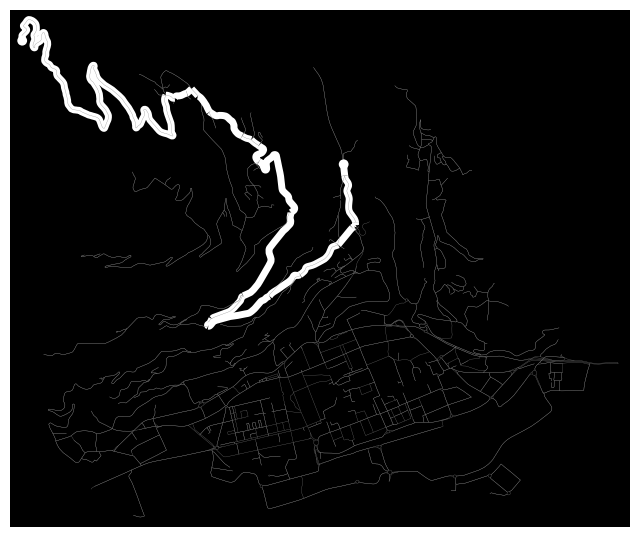
\includegraphics[width=\textwidth]{../plots/dijkstra/aosta/run04_DAO.png}
    \caption{Dijkstra (819 iter.)}
  \end{subfigure}\hfill
  \begin{subfigure}[b]{0.38\textwidth}
    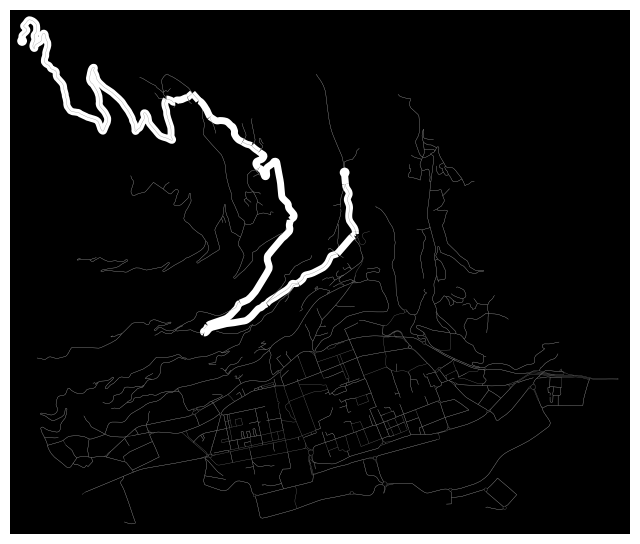
\includegraphics[width=\textwidth]{../plots/astar/aosta/manhattan/run04_AAOMAN.png}
    \caption{A* Manhattan (443 iter.)}
  \end{subfigure}
  \vspace{0.5em}
  \begin{subfigure}[b]{0.38\textwidth}
    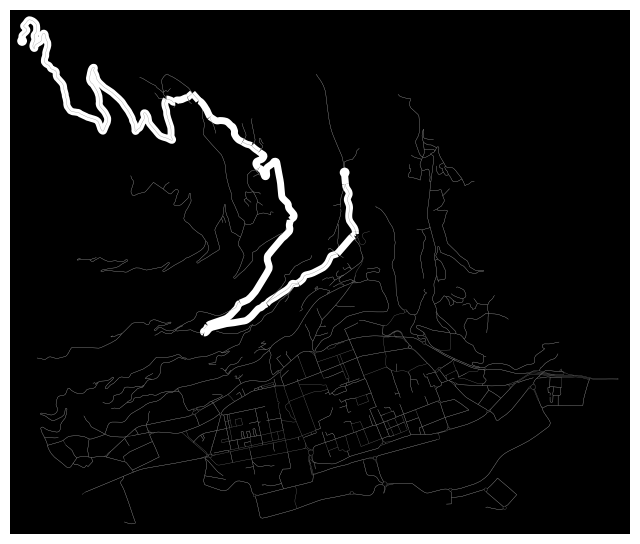
\includegraphics[width=\textwidth]{../plots/astar/aosta/euclidean/run04_AAOEUC.png}
    \caption{A* Euclidean (683 iter.)}
  \end{subfigure}\hfill
  \begin{subfigure}[b]{0.38\textwidth}
    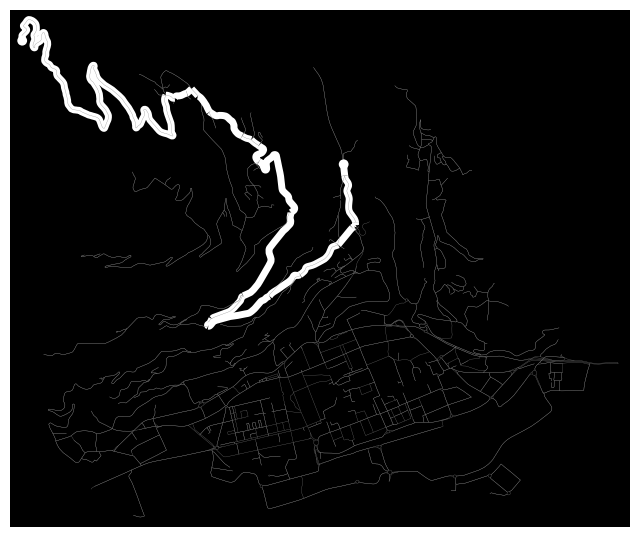
\includegraphics[width=\textwidth]{../plots/astar/aosta/haversine/run04_AAOHAV.png}
    \caption{A* Haversine (685 iter.)}
  \end{subfigure}
  \caption{Paths returned by each algorithm on run~4 in Aosta (9.67~km). All four paths are identical, verifying optimality.}
  \label{fig:paths_aosta}
\end{figure}

\subsection{Turin}

Table~\ref{tab:results_turin} reports the results for the Turin network, which is roughly 93 times larger than Aosta.
As in Aosta, path lengths are identical across all algorithms for every run, confirming optimality.
Figure~\ref{fig:paths_turin} shows the paths produced on run~4 (82.40~km).

\begin{table}[H]
  \centering
  \small
  \begin{tabular}{crrrrr}
    \toprule
    \textbf{Run} & \textbf{Dijkstra} & \textbf{A* Man.} & \textbf{A* Euc.} & \textbf{A* Hav.} & \textbf{Dist.~(km)} \\
    \midrule
    1  &  7\,867 &  4\,214 &  4\,712 &  4\,713 & 27.80 \\
    2  & 59\,949 & 15\,742 & 23\,299 & 23\,292 & 53.03 \\
    3  &  2\,767 &    615 &  1\,088 &  1\,090 & 12.19 \\
    4  & 47\,926 & 31\,027 & 35\,308 & 35\,307 & 82.40 \\
    5  &  3\,509 &  2\,519 &  2\,778 &  2\,779 & 16.83 \\
    6  & 37\,602 & 19\,658 & 22\,508 & 22\,515 & 18.61 \\
    7  & 24\,966 & 12\,773 & 14\,978 & 14\,982 & 26.19 \\
    8  &  4\,543 &  2\,068 &  2\,392 &  2\,393 & 10.11 \\
    9  & 58\,551 & 24\,062 & 39\,277 & 39\,280 & 81.57 \\
    10 & 23\,470 &  9\,382 & 12\,502 & 12\,532 & 32.30 \\
    \midrule
    \textbf{Avg} & 27\,115.0 & 12\,206.0 & 15\,884.2 & 15\,888.3 & \\
    \textbf{Impr.} & --- & $-55.0\%$ & $-41.4\%$ & $-41.4\%$ & \\
    \bottomrule
  \end{tabular}
  \caption{Iterations per run and average improvement over Dijkstra --- Turin (76\,483 nodes, 166\,951 edges).}
  \label{tab:results_turin}
\end{table}

\begin{figure}[H]
  \centering
  \begin{subfigure}[b]{0.38\textwidth}
    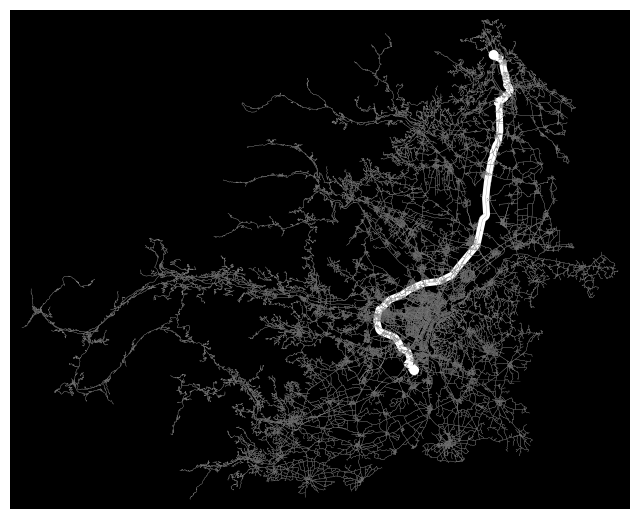
\includegraphics[width=\textwidth]{../plots/dijkstra/turin/run04_DTU.png}
    \caption{Dijkstra (47\,926 iter.)}
  \end{subfigure}\hfill
  \begin{subfigure}[b]{0.38\textwidth}
    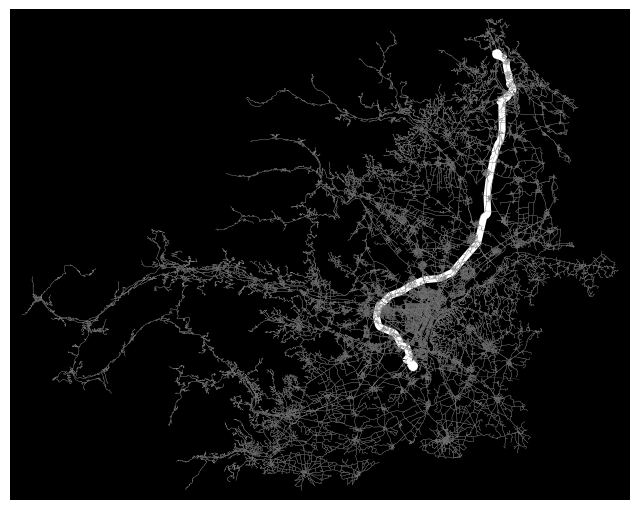
\includegraphics[width=\textwidth]{../plots/astar/turin/manhattan/run04_ATUMAN.png}
    \caption{A* Manhattan (31\,027 iter.)}
  \end{subfigure}
  \vspace{0.5em}
  \begin{subfigure}[b]{0.38\textwidth}
    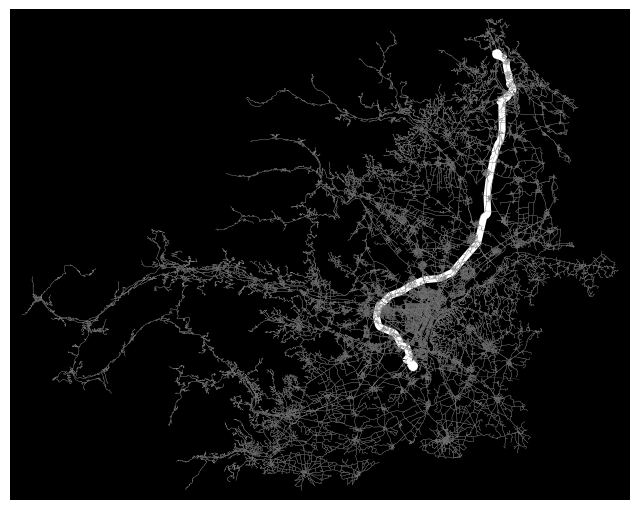
\includegraphics[width=\textwidth]{../plots/astar/turin/euclidean/run04_ATUEUC.png}
    \caption{A* Euclidean (35\,308 iter.)}
  \end{subfigure}\hfill
  \begin{subfigure}[b]{0.38\textwidth}
    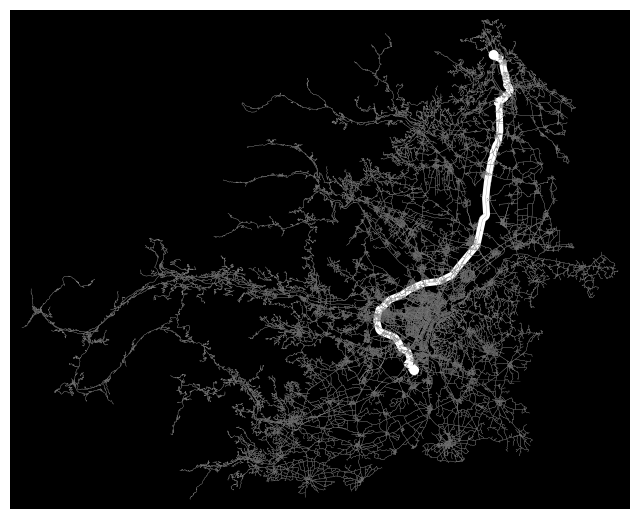
\includegraphics[width=\textwidth]{../plots/astar/turin/haversine/run04_ATUHAV.png}
    \caption{A* Haversine (35\,307 iter.)}
  \end{subfigure}
  \caption{Paths returned by each algorithm on run~4 in Turin (82.40~km). All four paths are identical, verifying optimality.}
  \label{fig:paths_turin}
\end{figure}

\subsection{Discussion}

Across both cities, all A* variants consistently reduce the number of iterations with respect to Dijkstra.
Path lengths are identical for all algorithm--run combinations, with the sole exception of A* Manhattan on run~3 in Aosta, where the returned path (3.67~km) is marginally longer than the optimal path found by Dijkstra (3.65~km), confirming the non-admissibility discussed in Section~\ref{sec:astar_design}.
For these particular origin-destination pairs the Manhattan heuristic achieves a $63.4\%$ reduction in Aosta and a $55.0\%$ reduction in Turin.
In both cases the reduction in absolute terms is substantial: in Turin, where Dijkstra explores an average of 27\,115 nodes before reaching the destination, A* Manhattan reduces this to 12\,206, a saving of roughly 15\,000 iterations per query.

Among the three heuristics, Manhattan consistently outperforms both Euclidean and Haversine in terms of iterations.
This can be attributed to the fact that the Manhattan distance satisfies $d_{\text{Man}} \geq d_{\text{Euc}}$ for any two points in the plane.
Normalising by $v_{\max}^{\star}$ yields a heuristic value that is always at least as large as the Euclidean one, which biases the search more aggressively towards the destination and reduces the number of nodes explored.
Note, however, that this also makes the Manhattan heuristic technically non-admissible: being larger than the Euclidean lower bound, it is not strictly guaranteed to underestimate the true remaining travel time, and path optimality cannot be formally proved for this variant.

The Euclidean and Haversine variants produce nearly identical results in both cities.
This is expected: at the spatial scale of a single city, the Earth's curvature is negligible, and the great-circle distance computed by the Haversine formula approximates the Euclidean distance on a flat plane.

Overall, the results demonstrate that A* can significantly reduce the computational effort required to find optimal paths in road networks, especially as the graph size increases.
The choice of heuristic also plays a crucial role, with the Manhattan distance providing the most effective guidance in this context.

% --- Appendices (optional) ---
%\appendix
%\section{Additional Material}

\end{document}